\section{Motivation}

General deep learing findings
DL boosted and is boosting performance and outcome in versatile applications. This spans large areas
text processing
image processing
audio processings
video processing for robotics
robotics itself, sensors actuators
analog signals
biological processes
explorative agent simulations
physical applications
computer graphics


before: spezialized algorithms, frameworks
now: models can be used interchangebly with adjustmens to fit the target task at hand.

the idea is learning itself - defined as.



universal function approximators, but highly dependent on the data as the model itself isnt worth anything before it has been adjusted (trained).
AGI - is of recent discussion where some models reach impressive results.



this brings us to the term generalization ...
Generalization
Wholistic models
what is needed for learning in the first place?

enough data can fit everything

still  problems, halluzinations, intransparency,

generalization can be tackeled at different stages of the medical image processing pipeline
model optimizing?
data curation is necessary?

can we do sth at training, model application?

Medical deep learing findings
as well as medical applications and processing of spezialized sensor data such as volumetric data as MRI CT.
especially for medical imaging where outcomes can have real world implications on fragile patients.
and can also be applied in the medical domain (SAM)

advent of deep learning in medical imaging




Definition of generalization

Gerneralization
    Data Acquisition
    Data Curation
    Model Building
    Model Application

What has been tried already? in those steps of the pipeline



\section{Objectives}

Objectives of this thesis
% TODO: What should go here?

Examine for all steps of the pipeline how available information / data in medical images can be utilized to improve the outcome

\section{Organisation and Contributions}

    \begin{figure}
        \label{fig:draft}
        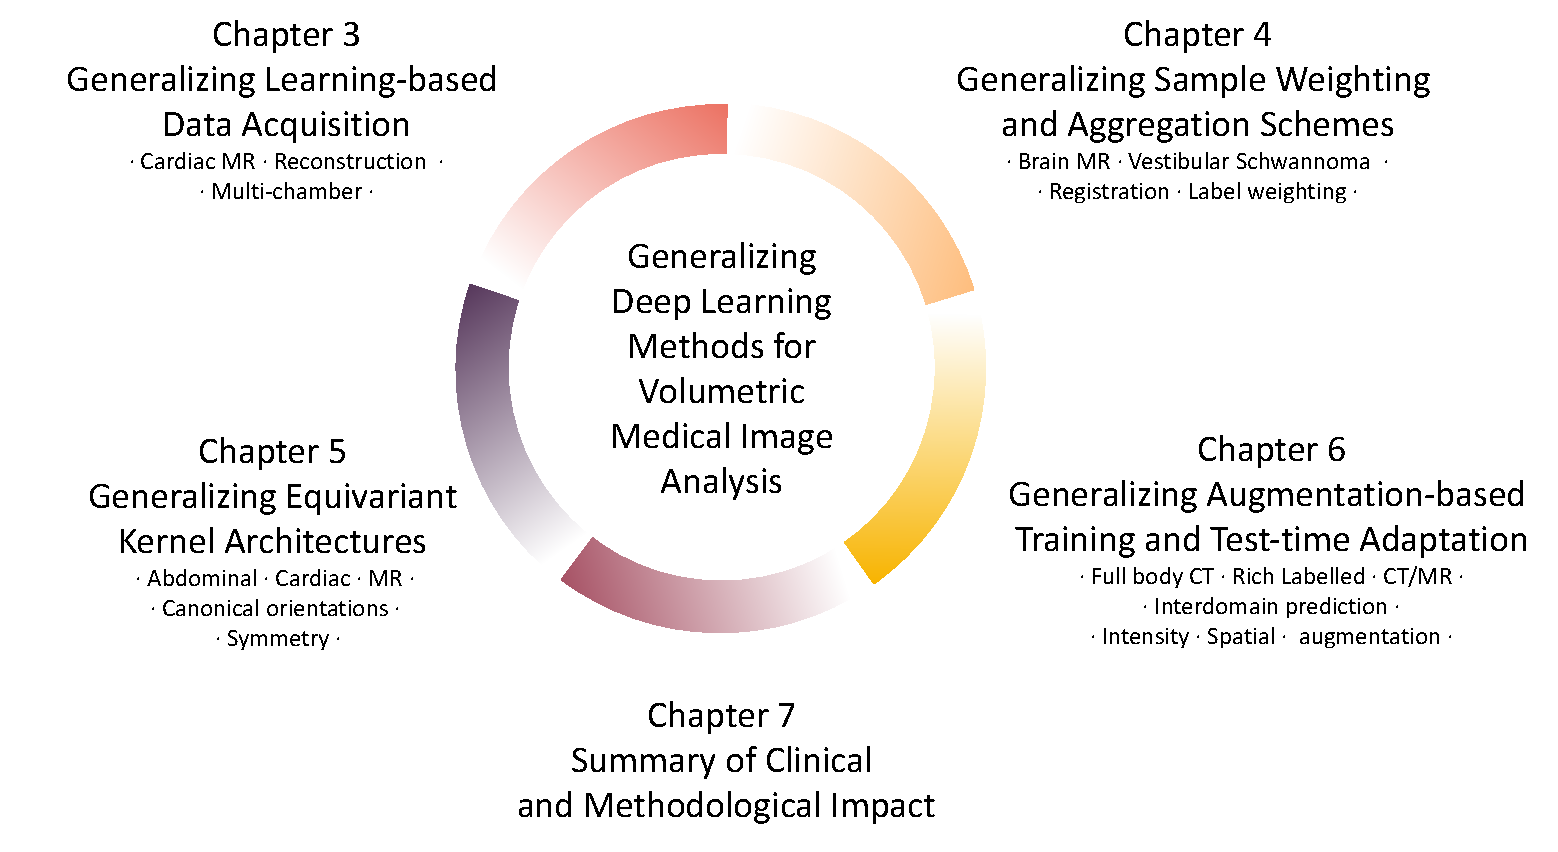
\includegraphics[width=\textwidth]{sections/01_introduction/figures/draft.pdf}
        \caption{Thesis draft}

    \end{figure}